\subsubsection{Fake rate application}

The application of the fake rates follows the same principles already used for the analysis that was performed
on the 8\TeV dataset.

In summary, a control region enriched in events with fake leptons, denoted as \emph{application region} in the following,
is selected by requiring that at least one of the selected leptons fails the tight lepton requirements.

The extrapolation from this control region to the signal region is performed by expressing the yields of events where $k$
leptons pass the full selection and $n-k$ fail it in terms of the yields of events with $n$ leptons among prompt and non-prompt
ones, efficiencies and fake rates, for $n=2$ or 3 and all possible values of $k$.\\

In two lepton events ($n=2$), the background contribution in the signal region can be expressed as:

\begin{equation*}
N_{pp}^\mathrm{bkg}  = \frac{f_1}{1\!-\!f_1} N_{pf}\ +\ \frac{f_2}{1\!-\!f_2} N_{pf}\ -\ \frac{f_1\,f_2}{(1\!-\!f_1)(1\!-\!f_2)} N_{ff}
\end{equation*}

under the approximation that the contribution of prompt leptons failing the selection can be neglected with respect to the contributions of non-prompt leptons.
It is worth noting that the event yield observed in the signal region does not affect the background prediction.\\

Following the same logic, the background prediction in the three lepton category is obtained by weighting
the events in the application region according to the following prescription:
\begin{itemize}
\item events with only one failing lepton are weighted by $f/(1\!-\!f)$, where $f$ is the fake rate evaluated on the kinematic quantities of the failing lepton;
\item events with two failing leptons ($i,j$) are weighted by $-f_if_j/((1\!-\!f_i)(1\!-\!f_j))$;
\item events with all three failing leptons are weighted by $f_1f_2f_3/((1\!-\!f_1)(1\!-\!f_2)(1\!-\!f_3))$.
\end{itemize}

A proof of the results presented above can be found in~\cite{CMS_AN_2013-159}.


\subsubsection{Closure tests and systematic uncertainties}

Closure tests are performed on simulated events in order to confirm that the methods described in the present Section are well suited to predict the reducible background after the event selection requirements.

A fake rate extracted from non-prompt leptons in QCD MC, selected inclusively, is first applied to 2lss semi-leptonic $\ttbar$ simulated events where at least one of the two selected candidates
fails the tight lepton requirements. Moreover, an alternative fake rate from non-prompt leptons in $\ttbar$ MC, selected inclusively as well, is applied to the same 2lss sample.

The test described above is performed in different event selections (separately for lepton flavors and analysis category). The difference in normalization between the two predictions, as well as their difference in the shape of the two kinematic discriminators against the $\ttbar$ and ttV backgrounds, are propagated as a systematic uncertainty to the fit used to extract the signal. Examples of the distributions can be found in Figures~\ref{fig:closure}.

The normalization uncertainties induced by the closure of the electron (muon) fake rate range from 10\% to 30\% (from 20\% to 40\%) depending on the analysis category, being larger in the b-tight case. Separate nuisance parameters account for the normalization in the b-loose and b-tight categories, and for different lepton flavors.

Shape uncertainties are evaluated at fixed normalization, and accounted for in the fit with linear distortions acting simultaneously on the two axes of the 2D BDT plane. The slope of the distortion typically ranges from 0.1 to 0.4, with separate nuisances for b-loose and b-tight categories, and for different lepton flavors.

\begin{figure}[htb]
        \centering 
        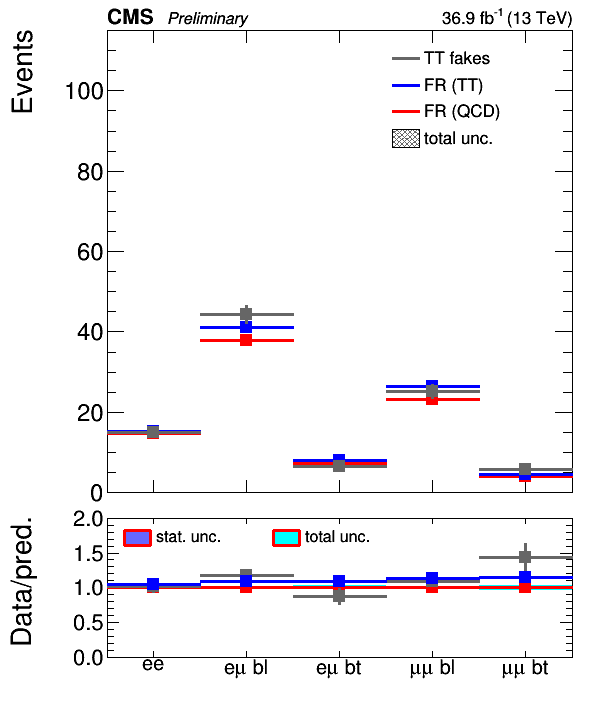
\includegraphics[width=0.32\textwidth]{plots_fakerate/application/2lss_SR_closuretest_flav/2lep_catIndex_nosign}
        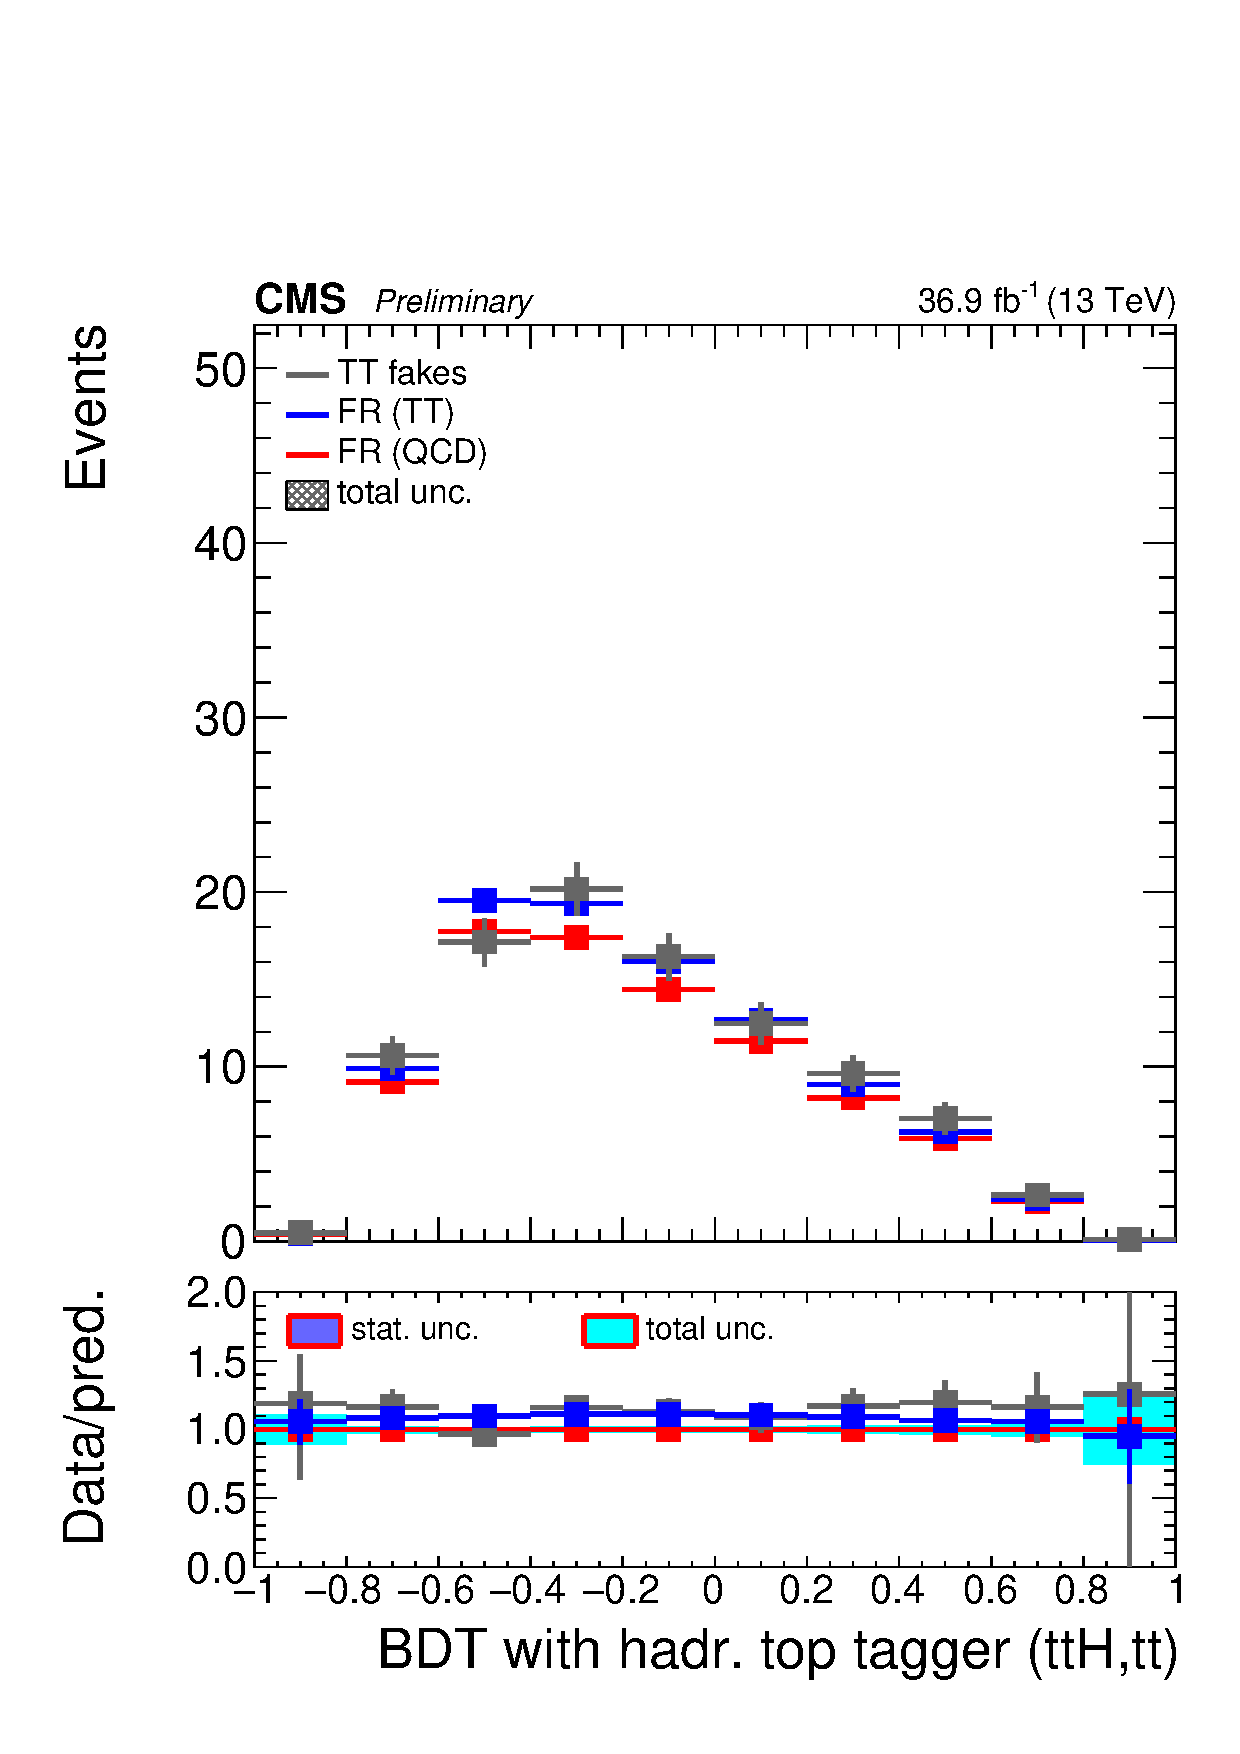
\includegraphics[width=0.32\textwidth]{plots_fakerate/application/2lss_SR_closuretest_flav/kinMVA_2lss_ttbar_withBDTv8}
        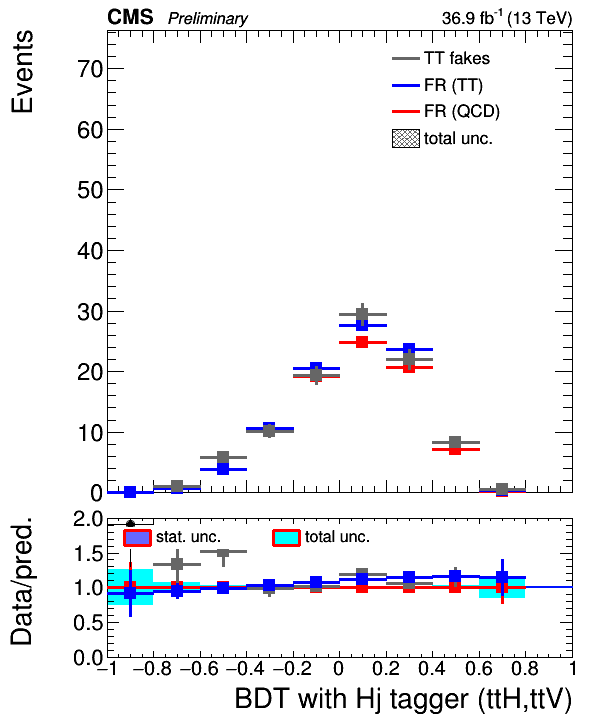
\includegraphics[width=0.32\textwidth]{plots_fakerate/application/2lss_SR_closuretest_flav/kinMVA_2lss_ttV_withHj}
        \caption{Normalization of event categories and distribution of background events in semi-leptonic $\ttbar$ events, compared with background predictions obtained in simulation using fake rates extracted in QCD and $\ttbar$ events.}
        \label{fig:closure}
\end{figure}

The uncertainty on the fake rate measurement is propagated to the background prediction introducing additional nuisances that vary both the background normalization via a coherent upwards or downwards shift of all bins in the fake rate map, and the background shape by introducing trends in the fake rate map as a function of the lepton $\pt$ and $|\eta|$, within the fake rate map uncertainty (Fig.~\ref{fig:FRvars_shape}), at constant normalization. This is done separately for electrons and muons.

\begin{figure}[htb]
        \centering 
        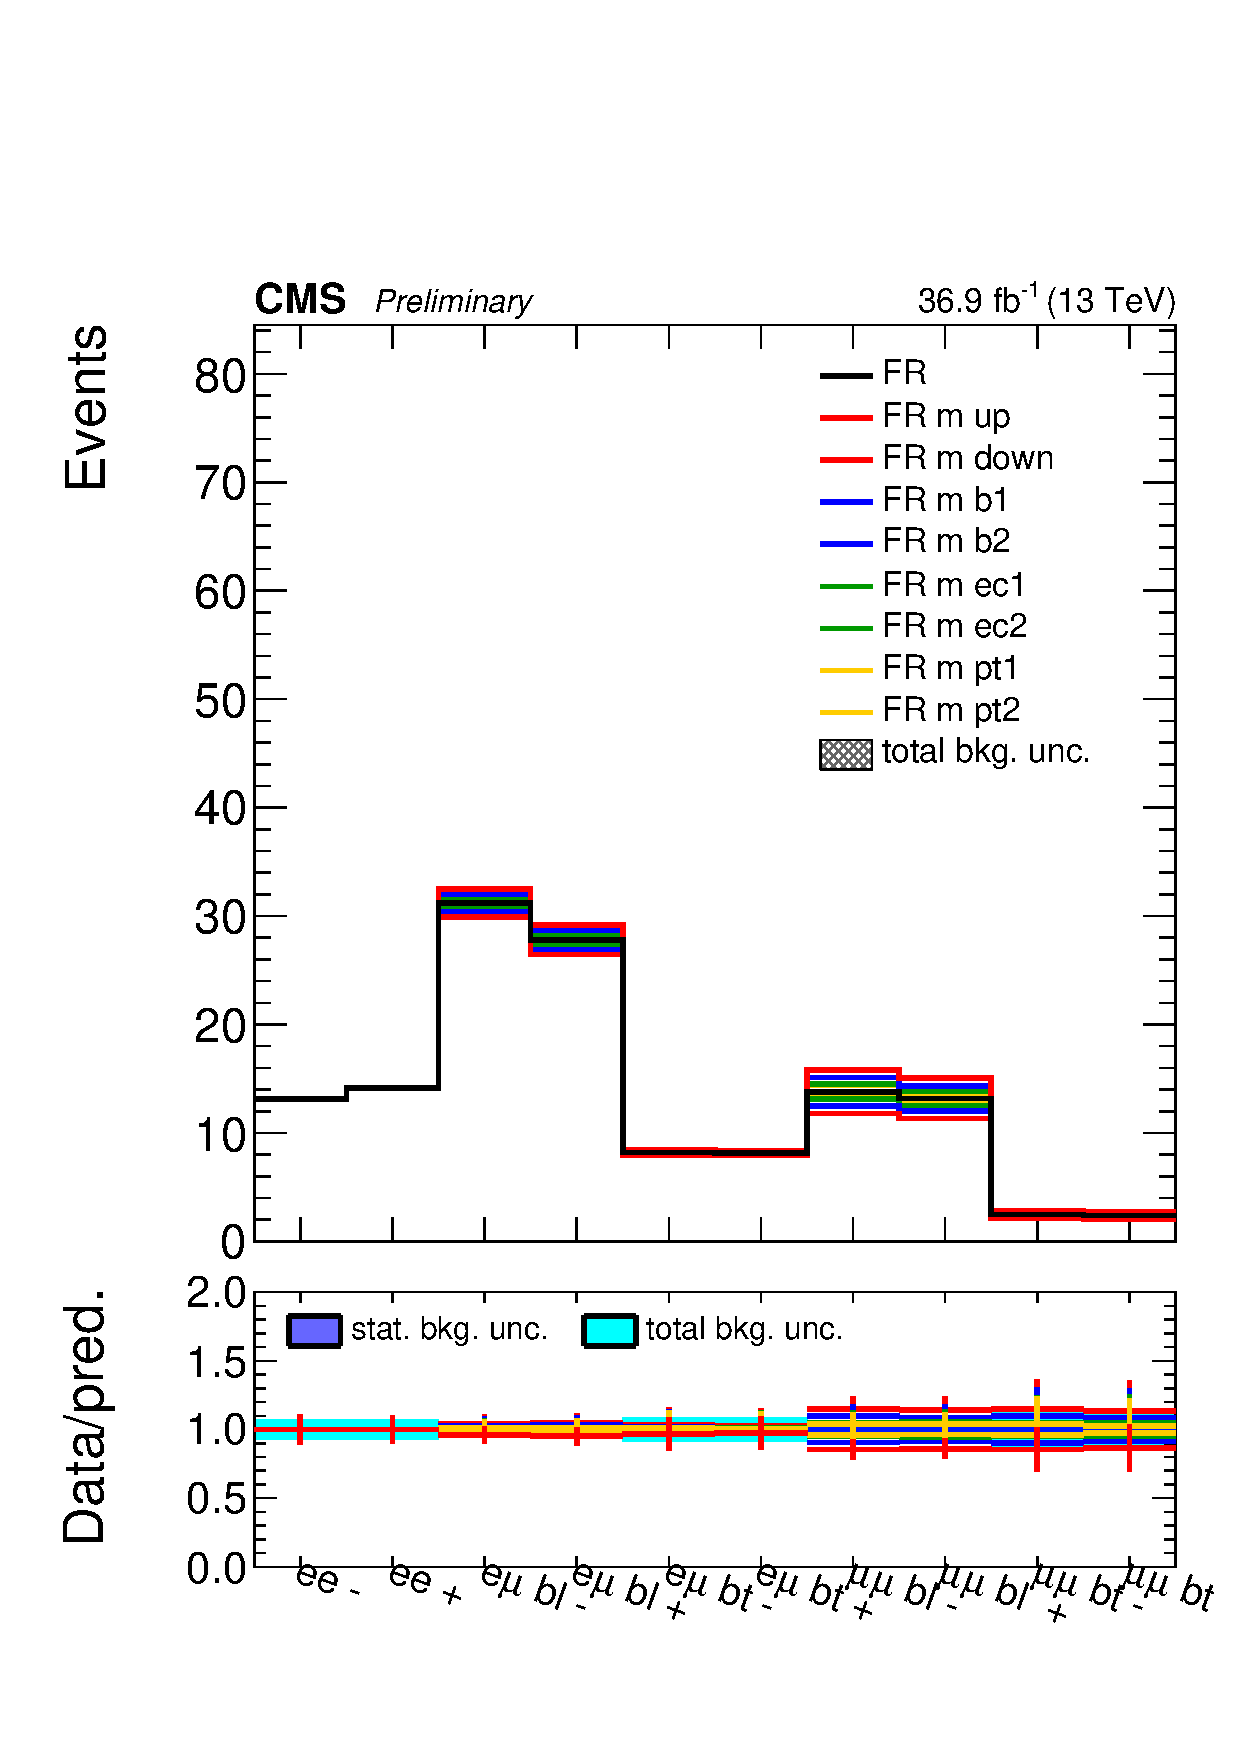
\includegraphics[width=0.32\textwidth]{plots_fakerate/application/2lss_SR_varsFR_m/2lep_catIndex}
        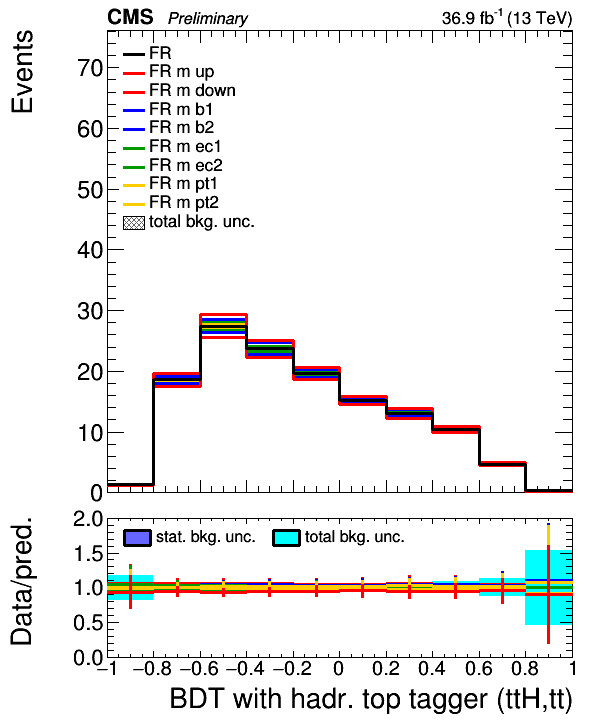
\includegraphics[width=0.32\textwidth]{plots_fakerate/application/2lss_SR_varsFR_m/kinMVA_2lss_ttbar_withBDTv8}
        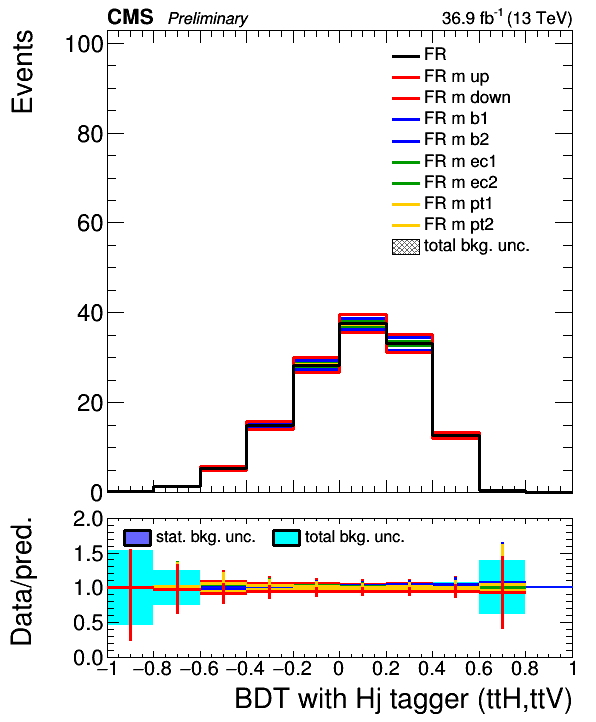
\includegraphics[width=0.32\textwidth]{plots_fakerate/application/2lss_SR_varsFR_m/kinMVA_2lss_ttV_withHj}\\
        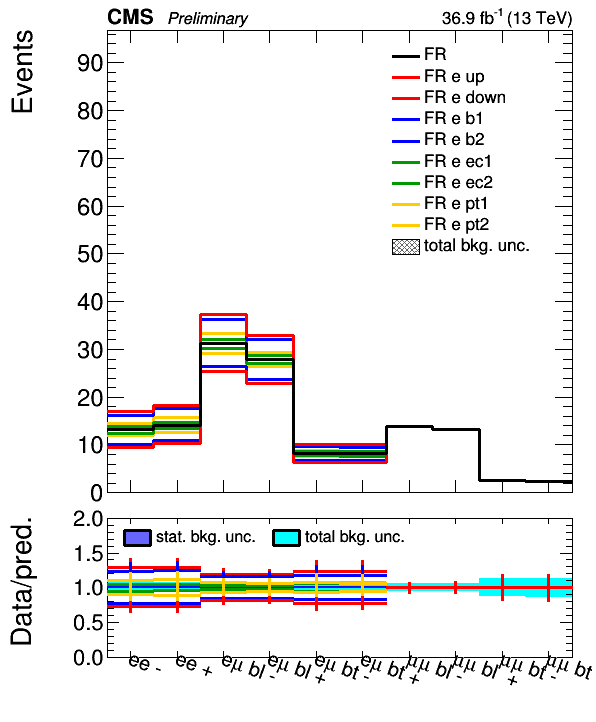
\includegraphics[width=0.32\textwidth]{plots_fakerate/application/2lss_SR_varsFR_e/2lep_catIndex}
        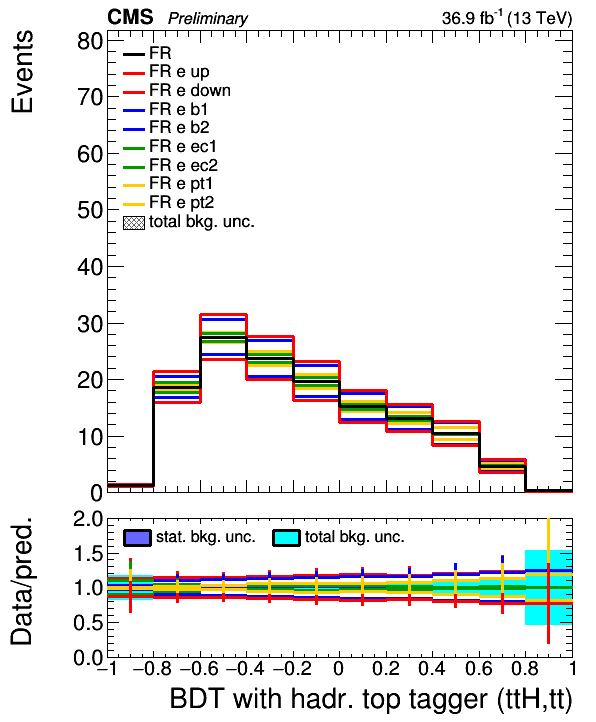
\includegraphics[width=0.32\textwidth]{plots_fakerate/application/2lss_SR_varsFR_e/kinMVA_2lss_ttbar_withBDTv8}
        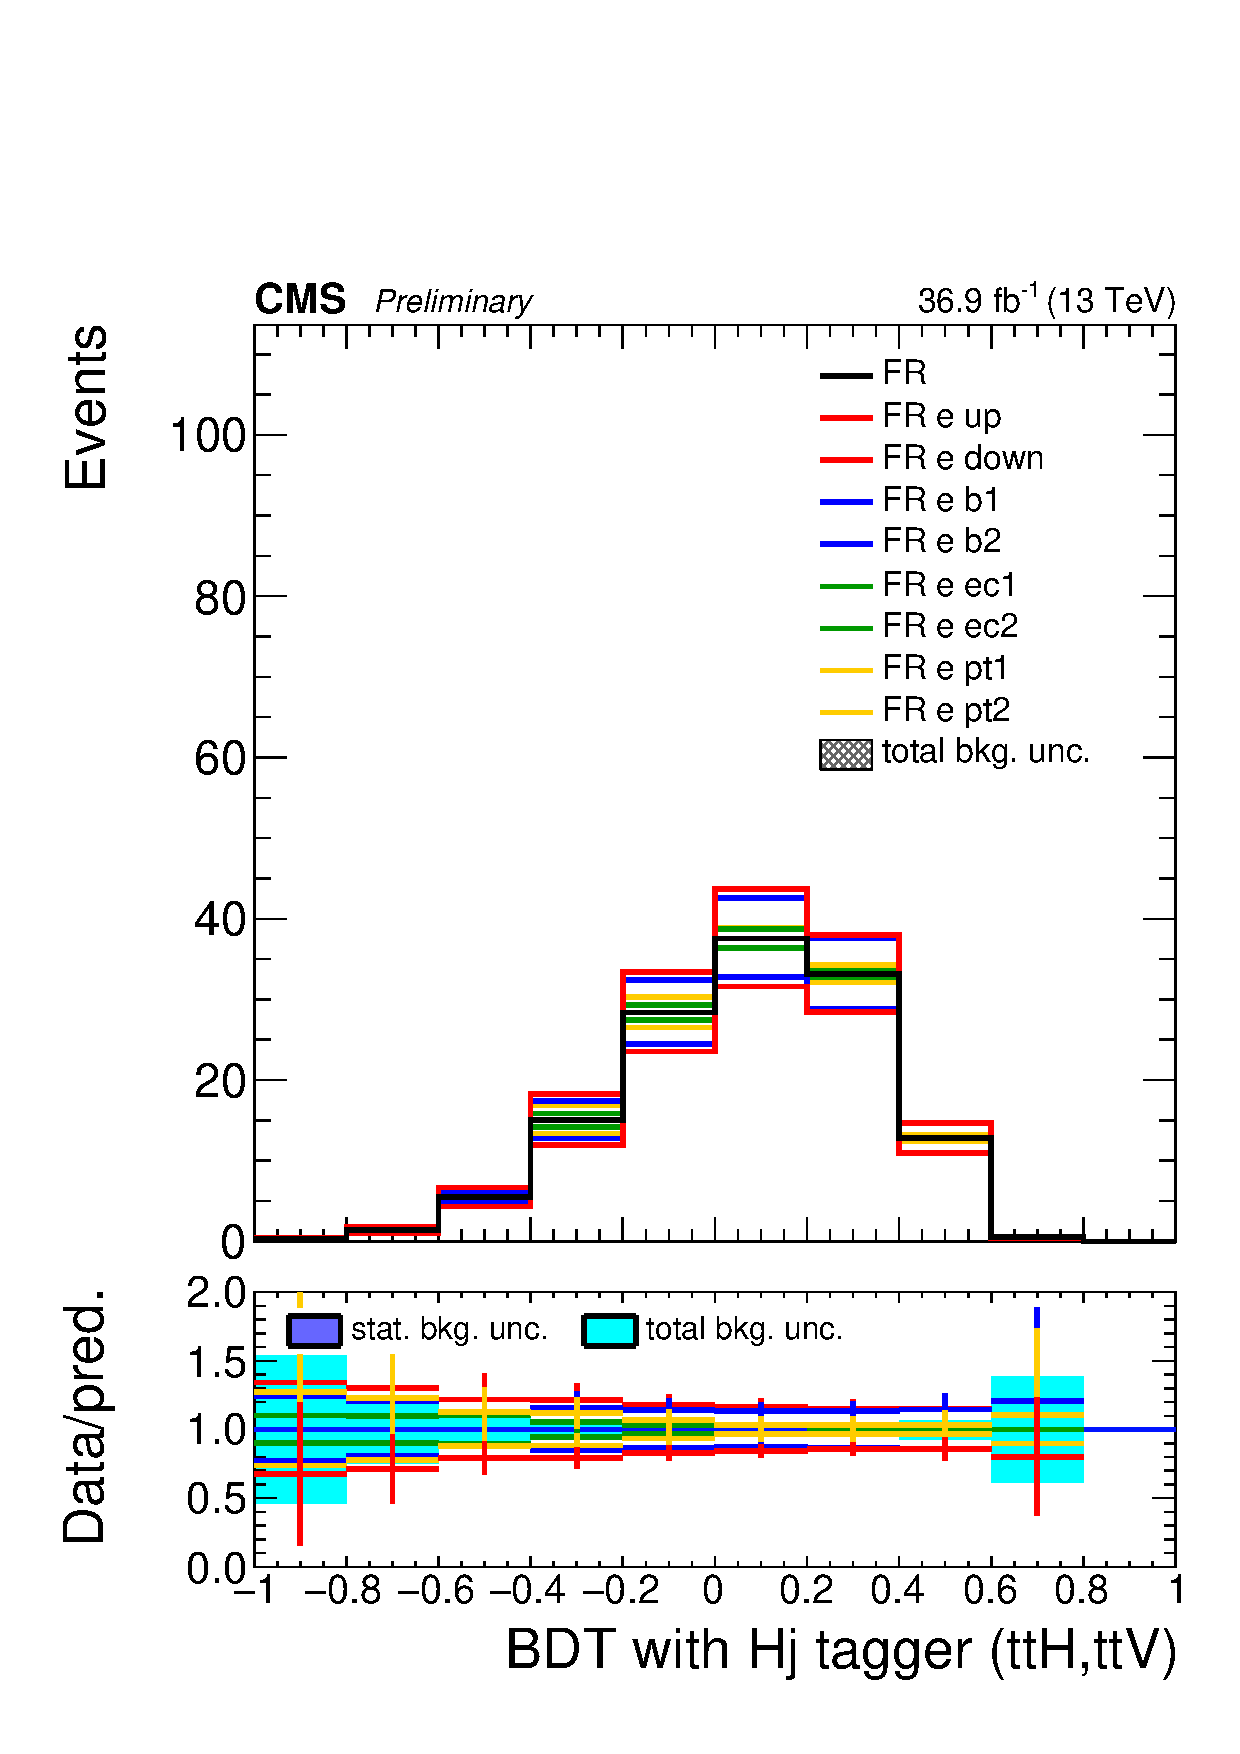
\includegraphics[width=0.32\textwidth]{plots_fakerate/application/2lss_SR_varsFR_e/kinMVA_2lss_ttV_withHj}
        \caption{Variation of background prediction induced by shifts and distortions of the measured data fake rate maps within their uncertainties. Red: global shift, blue: shift in barrel region only, green: shift in endcap region only, yellow: trend as a function of the lepton $\pt$. Top row is for muons, bottom one for electrons.}
        \label{fig:FRvars_shape}
\end{figure}

